\documentclass[a4paper, 10pt]{article}
\usepackage[UTF8]{ctex}
\usepackage{geometry}
\usepackage{graphicx}
\usepackage{setspace}
\usepackage{float}
\usepackage{listings}
\usepackage{xcolor}
\usepackage{multirow}
\lstset{
    numbers=left, 
    numberstyle= \tiny, 
    keywordstyle= \color{ blue!70},
    commentstyle= \color{red!50!green!50!blue!50}, 
    frame=shadowbox, % 阴影效果
    rulesepcolor= \color{ red!20!green!20!blue!20} ,
    escapeinside=``, % 英文分号中可写入中文
    xleftmargin=2em,xrightmargin=2em, aboveskip=1em,
    framexleftmargin=2em
} 
\geometry{left = 1.0 cm, right = 1.0cm, top = 2.0cm, bottom = 2.0cm	}
\title{编译原理第五章(一)}
\author{李鹏辉}

\begin{document}
\maketitle 

1.(5.1.1)对于图5-1中的SDD,给出下列表达式对应的注释语法分析树:
\begin{figure}[H]
\centering
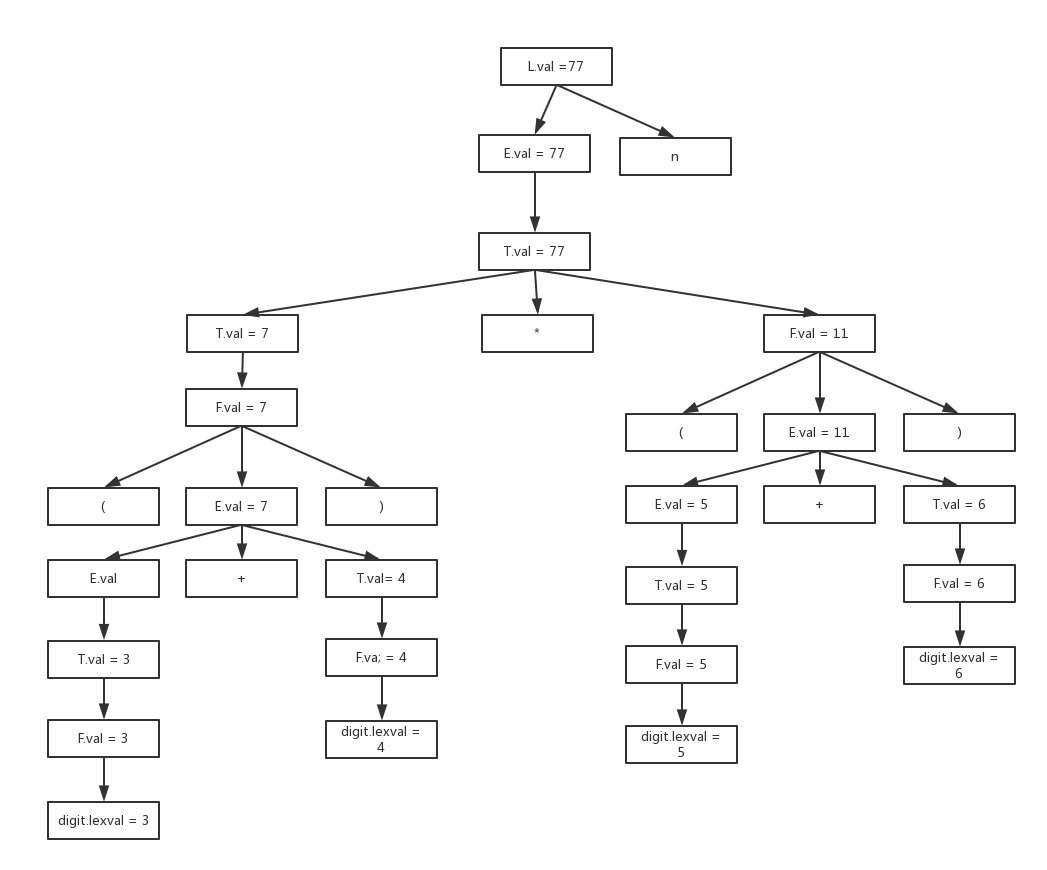
\includegraphics[scale=0.5]{chapter5_hw1}
\caption{Graph for FOR statement}
\end{figure}

2.(5.1.2)扩充图5-4中的SDD,使它可以像图5-1所示的那样处理表达式\\

\begin{table}[H]
\centering
\begin{tabular}{c|c}
\hline
\hline
Production & Samantic Rules\\ 
\hline
\multirow{2}{*}{$T \rightarrow FT' $} & $T'.inh = F.val$ \\
 & $T.val = T'.syn$ \\
\hline
\multirow{2}{*}{$T' \rightarrow *FT_1' $} & $T_1'.inh =T'.inh \times F.val$ \\
 & $T'.syn = T_1'.syn$ \\
 \hline
$T' \rightarrow \varepsilon $ &$T'.syn = T'.inh $ \\
\hline
$F\rightarrow digit $ &$ F.val = digit.lexval $ \\
\hline
$L \rightarrow En$ &$L.val E.val$ \\
\hline
\multirow{2}{*}{$E \rightarrow TE'$} & $E'.inh = T.val$ \\
&  $ E.val = E'.syn$ \\
\hline
\multirow{2}{*}{$E' \rightarrow +TE'$ }& $E'.inh = E'.inh + T.val $ \\
& $E'.syn = E'.syn$ \\
\hline
$F\rightarrow (E) $ &$F.val = E.val$ \\

\hline
\end{tabular}
\end{table}
注: L为起始符号,后五条为自行添加\\

3.(5.2.3)假设我们有一个产生式 $A \rightarrow $BCD,A、B、C、D这四个非终结符号都有两个属性:s是一个综合属性,i是一个继承属性。对于下面的每组规则,指出:(i)这些规则是否满足S属性定义的要求。(ii)这些规则是否满足L属性定义的要求。(iii)是否存在和这些规则一致的求值过程?\\

1) A.s = B.i + C.s

2) A.s = B.i + C.s 和 D.i = A.i + B.s

3) A.s = B.s + D.s

4) A.s = D.i, B.i = A.s + C.s, C.i = B.s 和 D.i = B.i + C.i

\begin{table}[H]
\centering
\begin{tabular}{c|c|c|c|c}
\hline
\hline
组数 & 1) & 2) & 3) & 4) \\
\hline
(1) & 不满足 & 不满足 & 满足 & 不满足\\
\hline
(2)&满足& 满足 & 满足 & 不满足\\
\hline
(3) & 存在 &存在 & 存在 & 不存在\\
\hline
\end{tabular}
\end{table}

\end{document}
